\documentclass[12pt]{report}
\usepackage[a4paper, bottom=1.5in]{geometry}
\usepackage{fancyhdr}
\usepackage{lastpage}
\usepackage{graphicx, wrapfig, subcaption, setspace, booktabs}
\usepackage[T1]{fontenc}
\usepackage[font=small, labelfont=bf]{caption}
\usepackage{fourier}
\usepackage[english]{babel}
\usepackage{sectsty}
\usepackage{url, lipsum}
\usepackage{enumitem}
\usepackage{float}
\usepackage{scrextend}
\usepackage{blindtext}
\usepackage[ruled,vlined]{algorithm2e}
\usepackage{algpseudocode}
\usepackage{tabularx}
\usepackage{booktabs}% http://ctan.org/pkg/booktabs

\newcommand{\tabitem}{~~\llap{\textbullet}~~}
\restylefloat{table}
\graphicspath{ {img/} }
\newcommand{\HRule}[1]{\rule{\linewidth}{#1}}
\renewcommand{\headrulewidth}{0pt}
\linespread{2}

\begin{document}
\begin{titlepage}
   \begin{center}
    	\normalsize \textbf{\uppercase{University of Waterloo}} \\
		Faculty of Mathematics \\
	\end{center}	
		\vspace*{\stretch{0.1}}
	\begin{center}
   		\LARGE \textbf{\uppercase{Achieving Quality through Automated Software Testing}}
	\end{center}
	\vspace*{\stretch{0.1}}
	\begin{center}
	   		\normalsize {Ultimate Software\\ San Francisco, California}	
	 
	\end{center}
	\vspace*{\stretch{0.1}}
	\begin{center}
	   		\normalsize {Prepared by\\
				Nicholas Westbury\\
				4A Computer Science\\
				ID 20550430\\
	   		 	\today
	   		 }
	\end{center}
\end{titlepage}

\newpage\noindent\thispagestyle{empty}
\linespread{1.2}
\LARGE\textbf{\uppercase{MEMORANDUM}} \normalsize
\vspace*{-10pt}
\begin{singlespacing}\noindent
\begin{labeling}{From:\ \ \ \ \ \ \ }
    \item [To:] Brian B.
    \item [From:] Nicholas Westbury
    \item [Date:] \today
    \item [Re:] Work Report: Achieving Quality Through Automated Software Testing
\end{labeling}
\end{singlespacing}
\vspace*{-10pt}
\HRule{1.5pt}
\begin{singlespacing}\noindent
I have prepared the enclosed report, "Achieving Quality through Automated Software Testing" for my fourth and final work report. The report is required by the Co-operative Education Program as part of Co-op degree requirements. \\ \\ \noindent 
As you know, I worked as part of the software development team for Perception, a survey tool that allows employers to get feedback and insights from algorithms that analyze the employee survey data using a mix of standard statistical and machine-learning methods. My primary duty this work term was to build features and tests for the Perception web application. As the product matures, focus is shifting from feature to stability work. Part of this effort is increased testing, forming the basis for this report. \\ \\ \noindent
As part of this process, the Faculty of Mathematics requests that you evaluate this report for command of topic and technical content/analysis. Your evaluation will be submitted to the Math Undergrad Office for evaluation. Fifteen percent of the weight is determined by your evaluation, the remainder by the faculty. The combined marks determine whether the report will receive credit. \\ \\
Thank you for your help in preparing this report,\\ \\ \noindent
\end{singlespacing}

\includegraphics[scale=0.55]{signature}
\linespread{2}

\newpage\thispagestyle{fancy}\sectionfont{\scshape}
\section*{Table of Contents}
\normalsize
\begin{enumerate}[label={},leftmargin=*,labelsep=2ex]
	\item Executive Summary \dotfill iv
    \item 1.0 Introduction \dotfill 1
    \item 2.0 Analysis \dotfill 2
    \begin{enumerate}[label*={},leftmargin=*,labelsep=2ex]
    	\item 2.1 Theory \dotfill 2
      	\begin{enumerate}[label*={},leftmargin=*,labelsep=2ex]
        	\item 2.1.1 Motivation \dotfill 2
        	\item 2.1.2 Why Testing is Difficult \dotfill 2
      	\end{enumerate}
      	\item 2.2 Types \dotfill 2
      	\begin{enumerate}[label*={},leftmargin=*,labelsep=2ex]
        	\item 2.2.1 White-Box Testing \dotfill 2
        	\item 2.2.2 Black-Box Testing \dotfill 2
      	\end{enumerate}
      	\item 2.3 Testing Levels \dotfill 3
      	\begin{enumerate}[label*={},leftmargin=*,labelsep=2ex]
        	\item 2.3.1 Unit Testing \dotfill 2
        	\item 2.3.2 Integration Testing \dotfill 2
        	\item 2.3.3 System Testing \dotfill 2
        	\item 2.3.4 Acceptance Testing \dotfill 2
      	\end{enumerate}
      	\item 2.4 Practical Implantation \dotfill 3
    \end{enumerate}
    \item 3.0 Conclusion \dotfill 12
    \item References \dotfill 13
\end{enumerate}
\fancyfoot[C]{ii}

\newpage\thispagestyle{fancy}\sectionfont{\scshape}
\section*{List of Figures}
\normalsize\cfoot{3aa}
\begin{enumerate}[label*={},leftmargin=*,labelsep=2ex,ref=\arabic*]
    \item Figure 1 --- Exponential Defect Cost Graph \dotfill 3
    \item Figure 2 --- Angular/Jasmine/Karma Logos \dotfill 9
	\item Figure 3 --- Current Testing Infrastructure \dotfill 10
\end{enumerate}

\section*{List of Tables}
\normalsize\cfoot{3aa}
\begin{enumerate}[label*={},leftmargin=*,labelsep=2ex,ref=\arabic*]
    \item Table 1 --- Unit Testing Pros and Cons \dotfill 7
    \item Table 2 --- Integration Testing Pros and Cons \dotfill 8

\end{enumerate}


\fancyfoot[C]{iii}

\newpage\thispagestyle{fancy}\sectionfont{\scshape}
\section*{Executive Summary}

This reports starts by looking at the theoretical motivation and objectives of testing and then considers some practical testing methods to attain these objectives. It will talk about the advantages, disadvantages, and trade-offs of a variety of software testing approaches and explains some of the considerations that goes into creating a broader company-wide testing strategy. After reading this report, the reader should understand why testing is important, why perfect testing is impossible, and be introduced to different classes of tests. Ultimately, the take-away will be understand the basis for testing and a sample implementation of this basis.

\fancyfoot[C]{iv}

%-------------------------------------------------------------------------------
% BODY
%-------------------------------------------------------------------------------

\newpage\thispagestyle{fancy}\sectionfont{\scshape}

% Reset the page counter
\setcounter{page}{1}
\fancyfoot[C]{\thepage}

\section*{1.0 Introduction}
\addcontentsline{toc}{section}{Introduction}
\par\indent
Software testing has always been a core pillar of building reliable computer programs. At its core, software testing is simply running a program and determining if the output is the expected behaviour based on requirements. It is composed of several linked activities: verifying software matches agreed-upon specifications, verifying software completeness, identifying defects in software that can take the form of feature, usability, or performance bugs [1]. As computer applications take an ever-growing roles in our lives, reliability and quality is crucial. \\ \par\noindent
The purpose of the report is to inform on a high-level about the why, what, and how of software testing. It will start by elaborating on why testing is important, background theory on different testing methods, and end with a sample practical application of these testing methods.

\newpage\thispagestyle{fancy}\sectionfont{\scshape}
\section*{2.0 Analysis}
\subsection*{2.1 Theory}
\noindent
Exclduing mission-critical applications, software testing has traditionally been seen as afterthought for startups that prioritize shipping features before worrying about stability. Nonetheless, in the long term, it is important to reduce programming bugs thereby increasing quality, leading to happier customers and more revenue. Automated testing leads to less manual regression testing lower cost and developement time.
\subsection*{2.1.1 Motivation: Cost}
\par\indent
The most easily measurable cost are the direct financial costs associated with software bugs. According to Tricentis, the cost was a staggering 1.1 trillion dollars in 2016 alone [2]. This figure includes direct expenses such as engineering costs to fix the bugs, the cost to customers being unable or impeded to use the product. Less frequently thought-about costs include the impact on the company's brand, customer loyalty, and level of annoyance customers report.
\par\noindent
Moreover, the later a bug is found and repaired, the more expensive it is to fix. A 2008 IBM report found that after a bug makes its way through the design, implementation, testing, customer beta test and finally post-production release, it is roughly 30 times more expensive compared to finding it during the design phase [3]. The earlier throughout testing is done, the cheaper it is. The next figure illustrates the exponential cost nature of defect the later it is found in the development process. 

\begin{center}
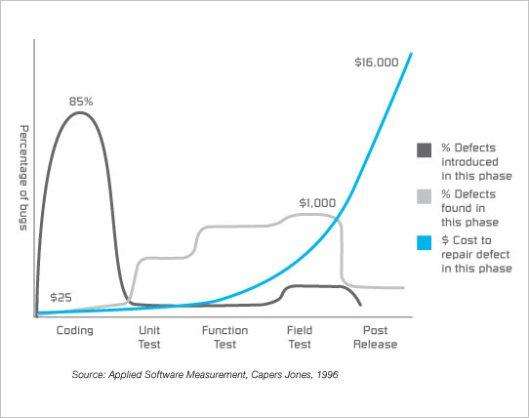
\includegraphics[scale=0.7]{cost-test}
\captionof{figure}{The cost of fixing a bug increases dramatically the later it is caught. [4]}
\end{center}
\par\noindent
In extreme cases, the costs are staggering. A high-profile case was Mariner 1, a 1962 NASA spacecraft with destination to Venus. Shortly after takeoff, it veered off course due to a software bug and \$18 million was lost [5]. Amazon Web Services went down for 4 hours causing nearly \$50 million dollars in lost revenue [6]. A software bug in the Therac-25 radiation machine caused larger-than-required dosage to be sent causing at least 3 deaths [7]. These examples are outliers, with thousands of smaller cases of bugs causing unexpected and expensive incorrect behaviour but they illustrate the need for software testing.

\subsection*{2.1.2 Motivation: Customer Happiness}
\par\noindent
Another common motivating factor is that better testing leads to happier customers. It is hard to measure customer happiness objectively but Medrad, a medical imaging equipment manufacturer, saw an annual revenue growth of 15\% for four years, which it attributed to a growing customer base after instituting a quality assurance (QA) program. Similarly, Johnson Controls, an automobile company, found as part of their QA efforts that every 1\% increase in customer satisfaction lead to a \$13 million positive impact on their bottom line [8].

\subsection*{2.1.2 Why Testing is Difficult}
\addcontentsline{toc}{section}{Introduction}
\par\noindent
Given that testing has benefits on both the company's bottom line and customer satisfaction, the natural question arises: why don't all software companies treat testing as a high priority? One reason is that testing is difficult. Even well-meaning companies that are willing to invest in QA might be afraid of the complexity.
\par\indent \\
To illustrate this point, consider the following simple pusedo-code:

\begin{algorithm}
	\caption{Simple Divison}
	\begin{algorithmic}
	
	\Function{divide}{a, b}
	  \State \Return a / b
	\EndFunction
	\end{algorithmic}
\end{algorithm}

\par\noindent
The number of aspects there is to analyze for test purposes is virtually limitless. For the snippet above, a type-conscience programmer might ask what types are $a$ and $b$ expected to be? Are they integers, floating-point numbers, or could they even be complex types like imaginary numbers or could $a$ be an array and $b$ an integer? Are these considerations that we should test for or these assumptions fair to make given the domain of the system? Do we need to test for every combination of number or is it sufficient to test certain edge cases? The answer to these questions will depend on an application's own error tolerance. \\

\par\noindent
Language-specific considerations also need to be taken into account. For example, python2 and C will return the floor when dividing integers. For example, $1$ divided by $2$ gives $0$. However, python3 will do float division with integers so $1 / 2 = 0.5$. A computer scientist might also point out edge cases when the result exceeds the $[-2^{31}, 2^{31}-1]$ range for 32-bit signed integers leading to under or overflow. Finally a mathematician might ask what would happen for the cases $a/0$ or $0/0$. The amount of knowledge and proper discretion required to test even trivial functions is very high. So high in fact that throughout software testing through mathematical proofs is reserved for mission-critical applications such as space exploration or medical. It is unnecessary and wasteful to test every case for most applications.

\section*{2.2 Types}

Traditionally, testing can be divided into two large categories: white and black box testing. White-box testing refers to testing when the implementation is known whereas black-box testing is testing where the code is unknown and product-behaviour testing is done. Each category can be further sub-divided into more specific categories.

\subsection*{2.2.1 White-box Testing}
\par\noindent
White-box includes any tests where the implementation is known to the developer. It is done at the unit testing phase. White-box testing has some advantages and disadvantages compared to black-box testing. 

\par\noindent
Generally white-box tests are more thorough than black-box since developers can put emphasis on more complex sections of the code. With knowledge of the underlying code, developers can test the code they know is most complex and therefore more risky. For this reason, performance issues are more easily identified here. Automating the tests is easier when the implementation is known.

\par\noindent
There are downsides too. For one, only a programmer is able to write tests. The number of inputs can frequently be too high to test throughly and may not be how the software would be used by a cusomter. White-box testing also has bias to the existing code-base and is generally worst at finding faults rather than testing existing behaviour.

\subsection*{2.2.2 Black-box Testing}
\par\noindent
Black-box is roughly the opposite of white-box testing. A tester knows \textit{what} the software should do but not \textit{how} it does it. It has the benefit of being able to be tested by anyone even without particular programming knowledge. They are closer to the product specification so it can be easier to find business-use edge-cases, but harder to find code edge-cases compared to white-box testing.

\section*{2.3 Testing Phases}
\par\noindent
Different phases of testing are appropriate for different degrees of specificity of a software testing. Each has its advantages and drawbacks and therefore the phases are often combined as part of a testing pipeline.

\subsection*{2.3.1 Unit Testing}
\par\noindent
Unit tests code on a functional-level. Generally they are written to ensure function or class-level behaviour is correct. A unit test minimally a single branch of logic and test the most complex or edge cases. Multiple unit tests should ideally cover every logical branch. Unit testing is intented to be used along with other testing method to complete a full testing strategy.

\begin{table}[ht]
\begin{tabularx}{\linewidth}{>{\parskip1ex}X@{\kern4\tabcolsep}>{\parskip1ex}X}
\toprule
\hfil\bfseries Pros & \hfil\bfseries Cons
\\\cmidrule(r{3\tabcolsep}){1-1}\cmidrule(l{-\tabcolsep}){2-2}

%% PROS, seperated by empty line or \par
$\bullet$ Simple to write\par
$\bullet$ Can be written independently of other code\par
$\bullet$ Serve as specification to other developers by giving concrete examples on how to use a particular function\par
$\bullet$Can be run in parallel because all external integration is mock\par
$\bullet$Easy to pinpoint exact line of broken code\par

&

%% CONS, seperated by empty line or \par
$\bullet$ Misleading code coverage because 100\% unit test coverage doesn't correspond to complete test coverage \par
$\bullet$ Doesn't cover interaction between components \par

\\\bottomrule
\end{tabularx}
\caption{Unit testing pros and cons}
\end{table}
\vspace{-10pt}
\subsection*{2.3.2 Integration Testing}
\par\noindent
Integration testing tests interaction between individual components with respect to a software specification. It combines unit-tested modules and tests the interaction between them.

\begin{table}[ht]
\begin{tabularx}{\linewidth}{>{\parskip1ex}X@{\kern4\tabcolsep}>{\parskip1ex}X}
\toprule
\hfil\bfseries Pros & \hfil\bfseries Cons
\\\cmidrule(r{3\tabcolsep}){1-1}\cmidrule(l{-\tabcolsep}){2-2}

%% PROS, seperated by empty line or \par
$\bullet$ Closer to testing the application with user requirements 

&

%% CONS, seperated by empty line or \par
$\bullet$ Can be challenging to separate unit-test into integration tests    dependent on code structure
$\bullet$ Not as easy to trace-down mistakes compared to unit tests

\\\bottomrule
\end{tabularx}
\caption{Integration testing pros and cons}
\end{table}

\subsection*{2.3.3 System Testing}
\par\noindent
System testing is a class of black-box testing where the program requirements are tested based on the product requirements. System testing is done on the completed overall system.

\subsection*{2.3.4 Acceptance Testing}
\par\noindent
The final testing phase is done by real users. It will be the most accurate test because run tests in real environments. It is often the last step before a product release.


\section*{2.4 Sample Practical Implementation}
\par\noindent
At work, our testing stack consists of a few different technologies. The primary technologies are Jasmine/Karma for client-side unit and integration testing, Frisby for backend API system testing, nosetests for python unit testing, and Selenium for system testing. The choice of these particular technologies is specific to our software stack but is illustrative of a well-rounded testing strategy.

\par\noindent
Jasmine and Karma are the testing framework and test runner that allow for unit-testing JavaScript code. We have framework-specific testing to allow Angular modules to be broken down into their natural components: controllers, services, and directives. These are akin to classes in object-oriented languages. Testing these components as a unit instead of individual function has the advantage that they are often closely coupled and directly dependent on another, making the testing closer to what is being run. One frustration is that these unit test require a considerable amount of mocking to seperate an individual component.

\begin{center}

\includegraphics[scale=0.4]{karma}
\captionof{figure}{Angular/Jasmine/Karma is a popular testing stack for frontend testing. [9]}
\end{center}

\par\noindent
Python nosetests are similar to Jasmine and Karma unit tests but for the backend instead of the frontend. They are divided from each individual file into the three divisions of our server code: gateways, service, and endpoints. Python has a mature first-party testing framework and generally accomplishes the theoretical goals of unit tests to be discrete, independent, and complete. Nonetheless, one downside is the automated tests for database communication is lengthy because each unit tests clears the database.

\par\noindent
Frisby is used for system testing. It allows for HTTP requests to be made to different endpoints. For example, a test case could be to create a question and add it to a survey using the (\texttt{/api/create\_survey} and \texttt{/api/add\_survey\_question/1} endpoints). Its purpose is to test the backend endpoints.

\par\noindent
Finally, there is Selenium, a web browser automation tool. It allows for a realistic recreation of how the client would see and use the website. It is used for full system testing. It allows for nearly arbitrary complex tests but the downside it is considerable more difficult to write, and often more brittle than than other testing technologies. For example, a graphical overhaul would require re-writing Selenium test cases.

\par\noindent
Each of these technologies has their limitations but together they cover the full-spectrum of tests. Karma/Jasmine cover the frontend. Frisby/Nosetests cover the backend. Selenium acts as the bridge between them. The figure below visually illustrates where each technology fits in the overall testing strategy.

\begin{center}
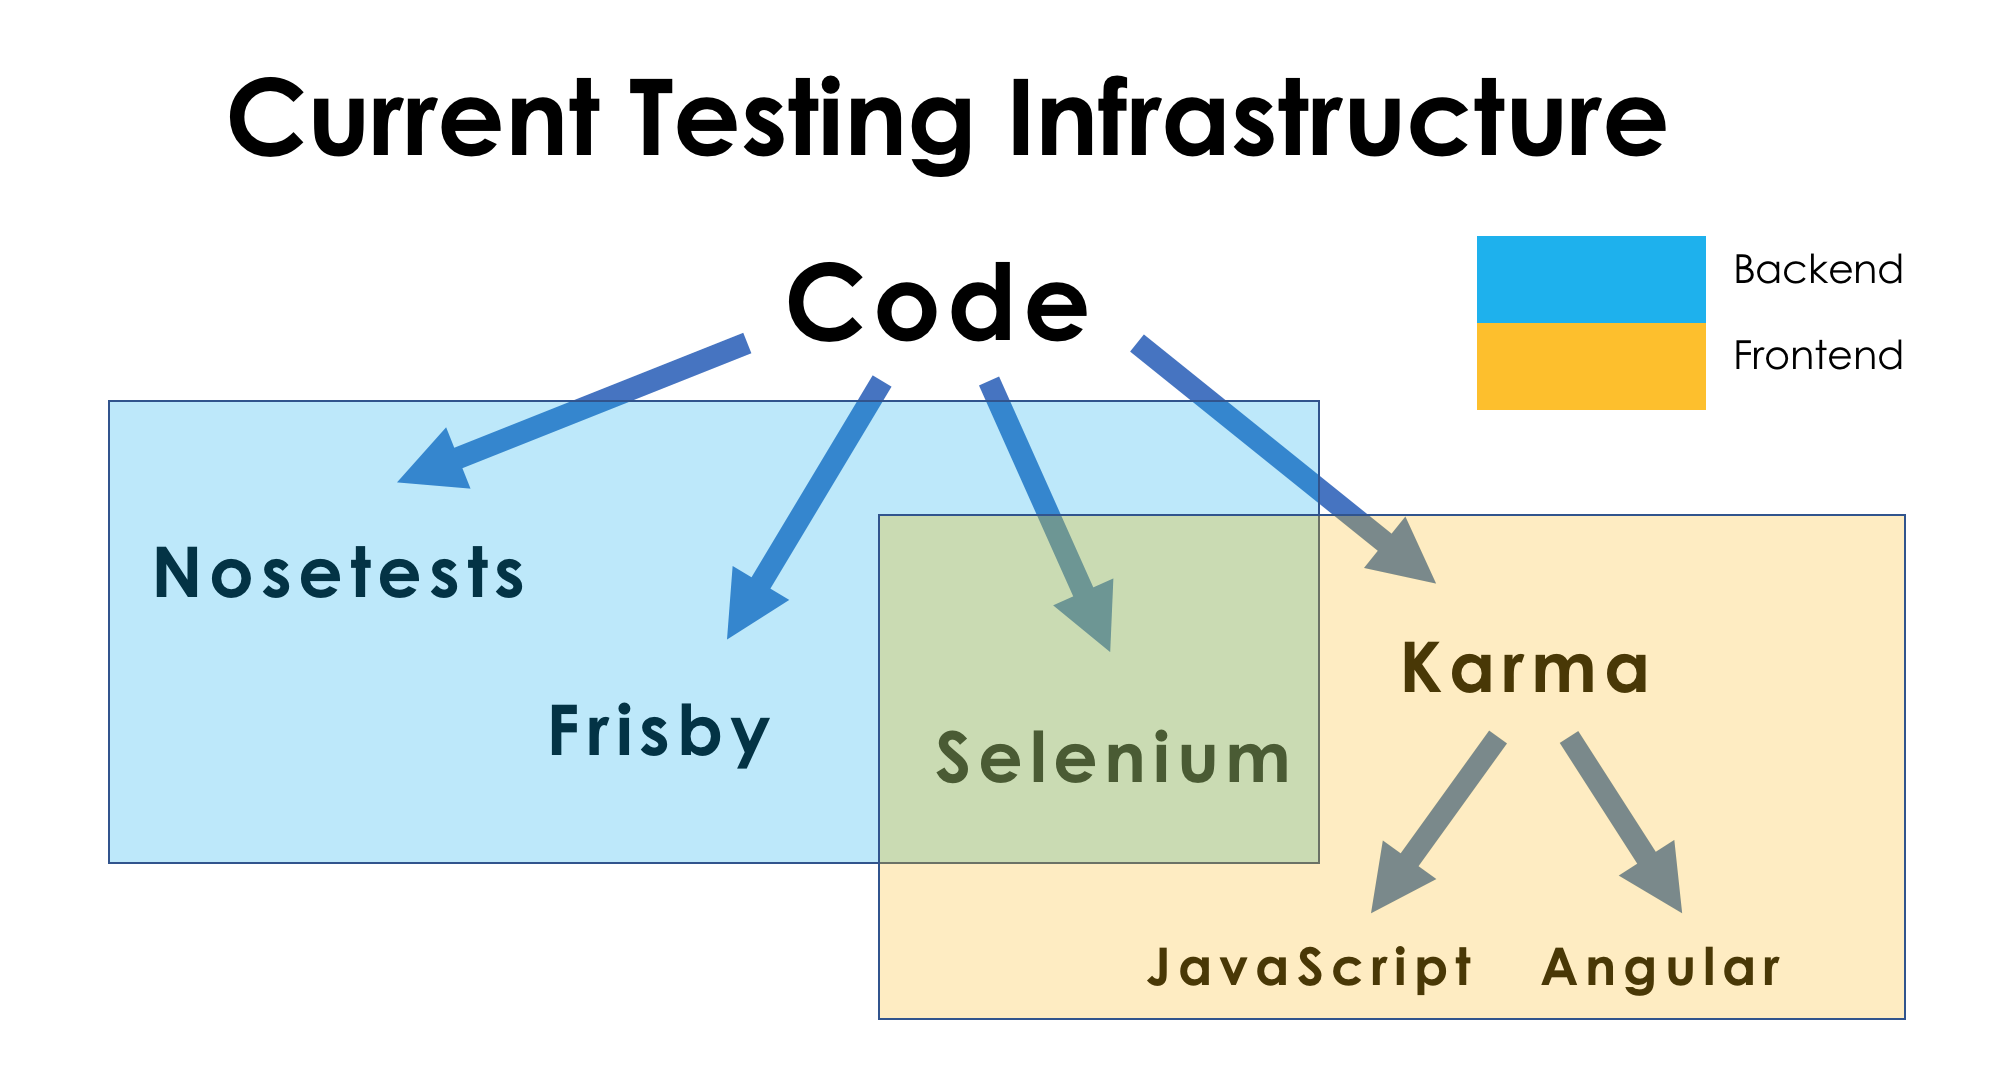
\includegraphics[scale=0.3]{infra}
\captionof{figure}{Four main technologies forming our testing infrastructure}
\end{center}

\newpage\thispagestyle{fancy}\sectionfont{\scshape}
\section*{3.0 Conclusion}
\addcontentsline{toc}{section}{Conclusion}
\par\noindent
As Perception matures, so does the importance for stability and thereby full-fledged automated tests. Increasing testing reduces the odds of a defect, increases customer satisfaction, and is correlated with increased revenues. Though perfect testing is practically impossible, the unit, integration, system, and acceptance testing pipeline is an effective way of having practical and useful tests. The explanation of our application of this theoretical model on practical product testing should highlight some of the strengths and weaknesses in the real-world. Automated software testing is a powerful tool towards achiving unparalleled quality.

 \noindent

%-------------------------------------------------------------------------------
% REFERENCES
%-------------------------------------------------------------------------------
\newpage
\section*{References}
\addcontentsline{toc}{section}{References}

\small
\begin{enumerate}
\item Pan, Jiantao. "Software Testing". Carnegie Mellon University, Spring 1999.st Newspaper, 25 Feb. 2012, https://users.ece.cmu.edu/\~koopman/des\_s99/sw\_testing/.

\item Tricentis. "Software Fail Watch: 2016 in Review". Tricentis, 2016. https://www.tricentis.com/resource-assets/software-fail-watch-2016/

\item International Business Machines. "Minimizing code defects to improve software quality and lower development costs", Oct. 2008. ftp://ftp.software.ibm.com/software/rational/info/do-more/RAW14109USEN.pdf

\item Manna, Antonella. "An Introduction to Testing in Production". Belatrix, 18 Aug. 2016. http://www.belatrixsf.com/blog/an-introduction-to-testing-in-production/

\item National Aeronautics and Space Administration (NASA). "Mariner 1", 2018. https://nssdc.gsfc.nasa.gov/nmc/spacecraftDisplay.do?id=MARIN1

\item Weise, Elizabeth. "Massive Amazon cloud service outage disrupts sites"
https://www.usatoday.com/story/tech/news/2017/02/28/amazons-cloud-service-goes-down-sites-scramble/98530914/

\item Levson, Nacy. "Medical Devices: The Therac-25". University of Washington, 1995. http://sunnyday.mit.edu/papers/therac.pdf

\item Turner, Jamie. "How Quality Impacts Your Bottom Line". SmartBear, 11 Apr. 2013. https://smartbear.com/blog/test-and-monitor/how-quality-impacts-your-bottom-line/

\item Rosa, Santiago. "Angular: Unit Testing Jasmine, Karma". 30 Nov. 2017. https://medium.com/frontend-fun/angular-unit-testing-jasmine-karma-step-by-step-e3376d110ab4
\end{enumerate}

\end{document}
